\documentclass{article}
\usepackage[utf8]{inputenc}
\documentclass[12pt]{article}
%\usepackage[left=3cm, right=2.5cm, top=2.5cm, bottom=2.5cm]{geometry}e}
\usepackage[utf8]{inputenc}
\usepackage[spanish,english]{babel}
\usepackage{apacite}
\usepackage[round]{natbib}
\usepackage{hyperref}
\usepackage{float}
\usepackage{svg}
\usepackage[margin = 1in, top=2cm]{geometry}% Margins
\setlength{\parindent}{2em}
\setlength{\parskip}{0.2em}
\usepackage{setspace} % Setting the spacing between lines
\usepackage{amsthm, amsmath, amsfonts, mathtools, amssymb, bm} % Math packages 
\usepackage{svg}
\usepackage{graphicx}
\usepackage{pgfplots}
\usepackage{epstopdf}
%\usepackage{subfig} % Manipulation and reference of small or sub figures and tables
\usepackage{hyperref} % To create hyperlinks within the document
\spacing{1.15}
\usepackage{appendix}
\usepackage{xcolor}
\usepackage{cancel}
\usepackage{enumerate}
\usepackage{subcaption}
\usepackage[shortlabels]{enumitem}


\usepackage[round]{natbib}
%\bibliographystyle{plainnat}
\bibliographystyle{apacite}


\newtheorem{defin}{Definition.}
\newtheorem{teo}{Theorem. }
\newtheorem{lema}{Lemma. }
\newtheorem{coro}{Corolary. }
\newtheorem{prop}{Proposition. }
\theoremstyle{definition}
\newtheorem{examp}{Example. }
\newtheorem{problem}{Problem}
% \numberwithin{problem}{subsection} 

\newcommand{\card}{\operatorname{card}}
\newcommand{\qiq}{\qquad \implies \qquad}
\newcommand{\qiffq}{\qquad \iff \qquad}
\newcommand{\qaq}{\qquad \textbf{and} \qquad}
\newcommand{\qoq}{\qquad \textbf{or} \qquad}
\newcommand{\settf}{\text{ \emph{:} }}
\newcommand{\chbox}{\makebox[0pt][l]{$\square$}\raisebox{.15ex}{\hspace{.9em}}}
\newcommand{\cchbox}{\makebox[0pt][l]{$\square$}\raisebox{.15ex}{\hspace{0.1em}$\checkmark$}}

\title{Problem Set 1}
\author{Mitchell Valdés-Bobes}
\date{September 14, 2020}

\begin{document}

\maketitle
\begin{problem}[\textbf{The Law of Supply}]



Suppose $k=3,$ and a firm uses goods one and two as inputs and produces good three as output. (Formally, $y \in Y$ requires $y_{1}, y_{2} \leq 0$.) For each of the following, either give an example showing it's possible or prove that it's impossible. (Feel free to use examples where $Y$ contains only a few points.)
\begin{enumerate}[(a)]
    \item If $p_{3}$ falls and $p_{1}$ and $p_{2}$ stay the same, can the firm's output $y_{3}$ go up?
    \item If $p_{1}$ rises and $p_{2}$ and $p_{3}$ stay the same, can the firm's output $y_{3}$ go up?
    \item (Harder:) If $p_{1}$ and $p_{2}$ both increase and $p_{3}$ stays the same, can the firm's output $y_{3}$ go up? What if $p_{1}$ and $p_{2}$ both increase by $10 \% ?$
\end{enumerate}
\end{problem}
\begin{proof}[Answer]
For this problem $p=(p_1, p_2, p_3)$  will represent old prices and $p'=(p'_1, p'_2, p'_3)$ new prices. $y\in Y^*(p)$ and $y'\in Y^*(p')$. The notation $a \cdot b$ refers to the scalar product of vectors, i.e.  $a \cdot b = \sum{a_ib_i}$
\newline
\newline
\textbf{Part(a)}
Suppose that:
\begin{equation}\label{pc1}
 p - p' = (0,0,p_3-p'_3) \qquad \text{where } p_3-p'_3>0    
\end{equation}
 
using optimality  we can guarantee that

$$y\cdot p \geq y'\cdot p$$
$$y' \cdot p' \geq y\cdot p'$$

adding the above inequalities we get

$$y\cdot p + y' \cdot p' \geq y'\cdot p  + y\cdot p'$$

which implies

$$(p-p')\cdot y \geq (p-p')\cdot y'$$

using \eqref{pc1}:

$$(p_3-p'_3)y_3 \geq (p_3-p'_3)y'_3$$

we can multiply this expression by the positive constant $1/(p_3-p'_3)$ without flipping  the inequality sign, therefore

$$y_3 \geq y'_3$$

this implies that the answer to the question is:

$$\boxed{\text{Under the price change described, the firm's output } y_{3}\text{ can't go up}}$$
\newline
\newline
\textbf{Part(b)}

Consider the following production set:

$$Y = \{(-5,-1,2), (-1,-6,3)\}$$

and prices

$$p=(1,2,4) \qquad p'=(2,2,4)$$

then

$$(-5,-1,2)\cdot p = 1 \text{ and } (-1,-6,3)\cdot p = -1 \qiq Y^*(p) = \{(-5,-1,2)\}$$

and

$$(-5,-1,2)\cdot p' = -4 \text{ and } (-1,-6,3)\cdot p' = -2 \qiq Y^*(p) = \{(-1,-6,3)\}$$

this is an example where $y_3<y'_3$ therefore the answer to the question is:
$$\boxed{\text{Under the price change described, the firm's output } y_{3}\text{ can go up}}$$
\newline
\newline
\textbf{Part(c)}
First we examine what it means to increase $p_1$ and $p_2$ and leave $p_3$ unchanged $(p_3'>p_3)$, then by optimality we will have

$$ -(p_1\cdot y_1+p_2\cdot y_2) + p_3\cdot  y_3 \geq -(p_1\cdot y'_1+p_2\cdot y'_2) + p_3\cdot  y'_3 \qiq p_1\cdot (y'_1 -y_1) + p_2\cdot (y'_2-y_2) \geq p_3\cdot (y'_3-y_3)$$
$$ -(p'_1\cdot y_1+p'_2\cdot y_2) + p_3\cdot  y_3 \leq -(p'_1\cdot y'_1+p'_2\cdot y'_2) + p_3\cdot  y'_3 \qiq p'_1\cdot (y'_1 -y_1) + p'_2\cdot (y'_2-y_2) \leq p_3\cdot (y'_3-y_3)$$
This means that
\begin{equation}\label{pc2}
p'_1\cdot (y'_1 -y_1) + p'_2\cdot (y'_2-y_2) \leq  p_1\cdot (y'_1 -y_1) + p_2\cdot (y'_2-y_2)
\end{equation}

since prices real non negative numbers we can write:

$$p_1' = (1+\alpha)p_1 \qaq p_2' = (1+\beta)p_2 \qquad \text{where } \alpha,\beta >0 $$ 

Then \eqref{pc2} is:

$$(1+\alpha)p_1\cdot (y'_1 -y_1) + (1+\beta)p_2\cdot (y'_2-y_2) \leq  p_1\cdot (y'_1 -y_1) + p_2\cdot (y'_2-y_2)$$

\begin{equation}\label{pc3}
\qiq \alpha p_1\cdot (y'_1 -y_1) + \beta p_2\cdot (y'_2-y_2) \leq  0
\end{equation}
This means that in principle we could construct an example where $y_3$ could go up.

Consider the following production set:

$$Y = \{(-5,-1,2), (-1,-6,3)\}$$

and prices

$$p=(100,200,400) \qquad p'=(200,225,400)$$

then

$$(-5,-1,2)\cdot p = 100 \text{ and } (-1,-6,3)\cdot p = -100 \qiq Y^*(p) = \{(-5,-1,2)\}$$

and

$$(-5,-1,2)\cdot p' = -425 \text{ and } (-1,-6,3)\cdot p' = -350 \qiq Y^*(p) = \{(-1,-6,3)\}$$

this is an example where $y_3<y'_3$ therefore the answer to the question is:
$$\boxed{\text{Under the price change described, the firm's output } y_{3}\text{ can go up}}$$

Now, if both $p_1$ and $p_2$ increase in the same proportion (in particular $10\%$) then we will have \eqref{pc3} with $\alpha=\beta$ which means:

\begin{align*}
    \alpha p_1\cdot (y'_1 -y_1) + \alpha p_2\cdot (y'_2-y_2) \leq  0 &\qiq  p_1\cdot (y'_1 -y_1) + p_2\cdot (y'_2-y_2) \leq  0 \\
    & \qiq p_1\cdot y'_1 + p_2\cdot y'_2 \leq p_1\cdot y_1 + p_2\cdot y_2 \\
    & \qiq -(p_1\cdot y'_1 + p_2\cdot y'_2) \geq -(p_1\cdot y_1+ p_2\cdot y_2)
\end{align*}

but consider the profits of $y$ and $y'$ under the original prices:

$$-(p_1\cdot y'_1 + p_2\cdot y'_2) + p_3 y_3 > -(p_1\cdot y_1+ p_2\cdot y_2) + p_3 y_3$$

and we know that the inequality is strict because we just have show that costs are lower and we are assuming that $y_3'>y_3$. But this contradicts the Weak Axiom of Profits Maximization; therefore the answer to the second part of the question is:

$$\boxed{\text{When prices } p_1, p_2 \text{both increase in 10\%  the firm's output } y_{3}\text{ can't go up}}$$

\end{proof}

\begin{problem}
Consider the following two "datasets":
$$
\begin{array}{cc|cc}
{\text { Dataset 1 }}  & &  {\text { Dataset 2 }} & \\
p & y(p) & p & y(p) \\
\hline(7,4) & (-20,40) & (7,4) & (-20,40) \\
(5,5) & (-50,60) & (5,5) & (-40,70) \\
(4,8) & (-70,90) & (4,8) & (-70,90)
\end{array}
$$
For each one, determine whether the three observations are consistent with a profit-maximizing firm. If not, explain why not. If so, draw or describe:

\begin{enumerate}[(a)]
    \item the smallest production set that can rationalize the data.
    \item the smallest convex production set with free disposal and the shutdown property that can rationalize the data.
    \item the largest production set that can rationalize the data
\end{enumerate}

\end{problem}

\begin{proof}[Answer]
\textbf{Dataset 1}

We can draw the points $y(p)$ in the plane and the corresponding hyperplane for each price vector-point combination:

\begin{figure}[!tbp]
  \centering
  \begin{subfigure}{0.45\textwidth}
    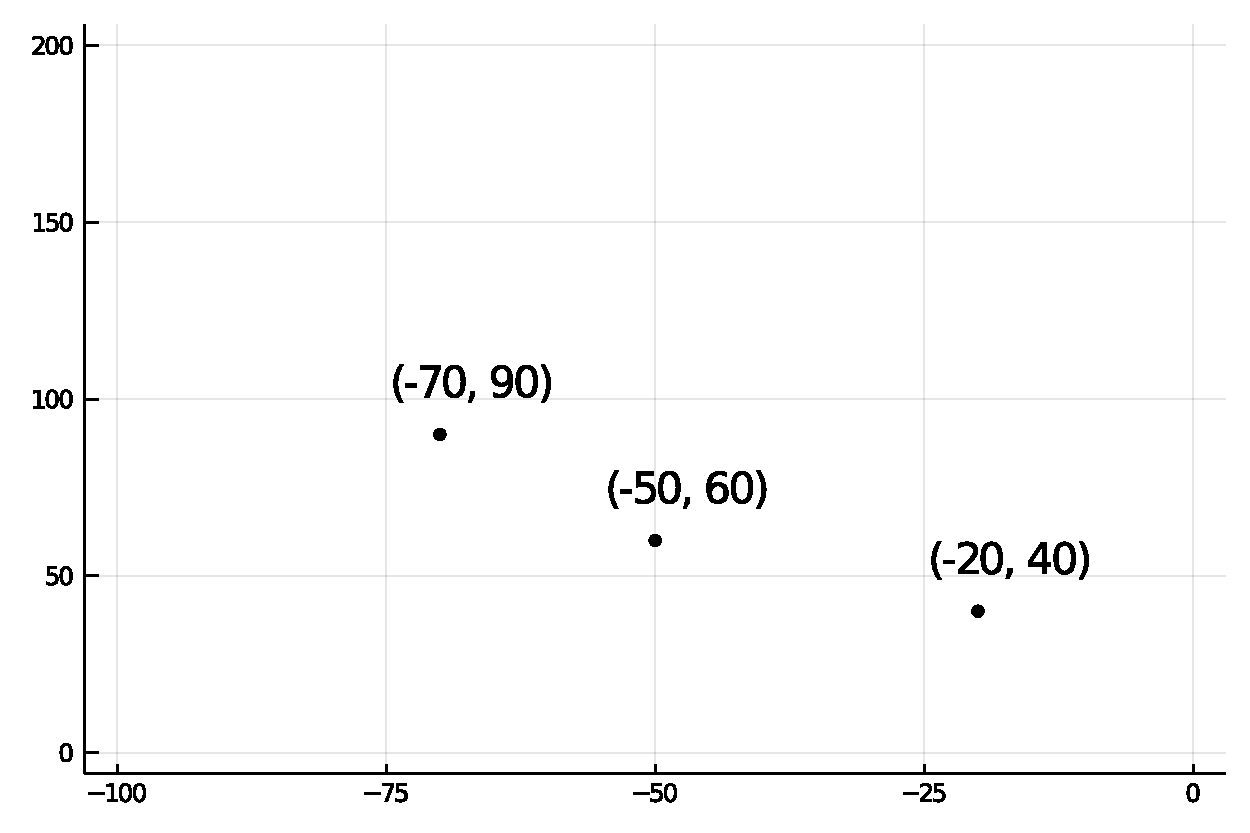
\includegraphics[width=0.97\textwidth]{Problem Set 1 Files/y_i_1.pdf}
    % \caption{Flower one.}
  \end{subfigure}
  \hfill
  \begin{subfigure}{0.45\textwidth}
    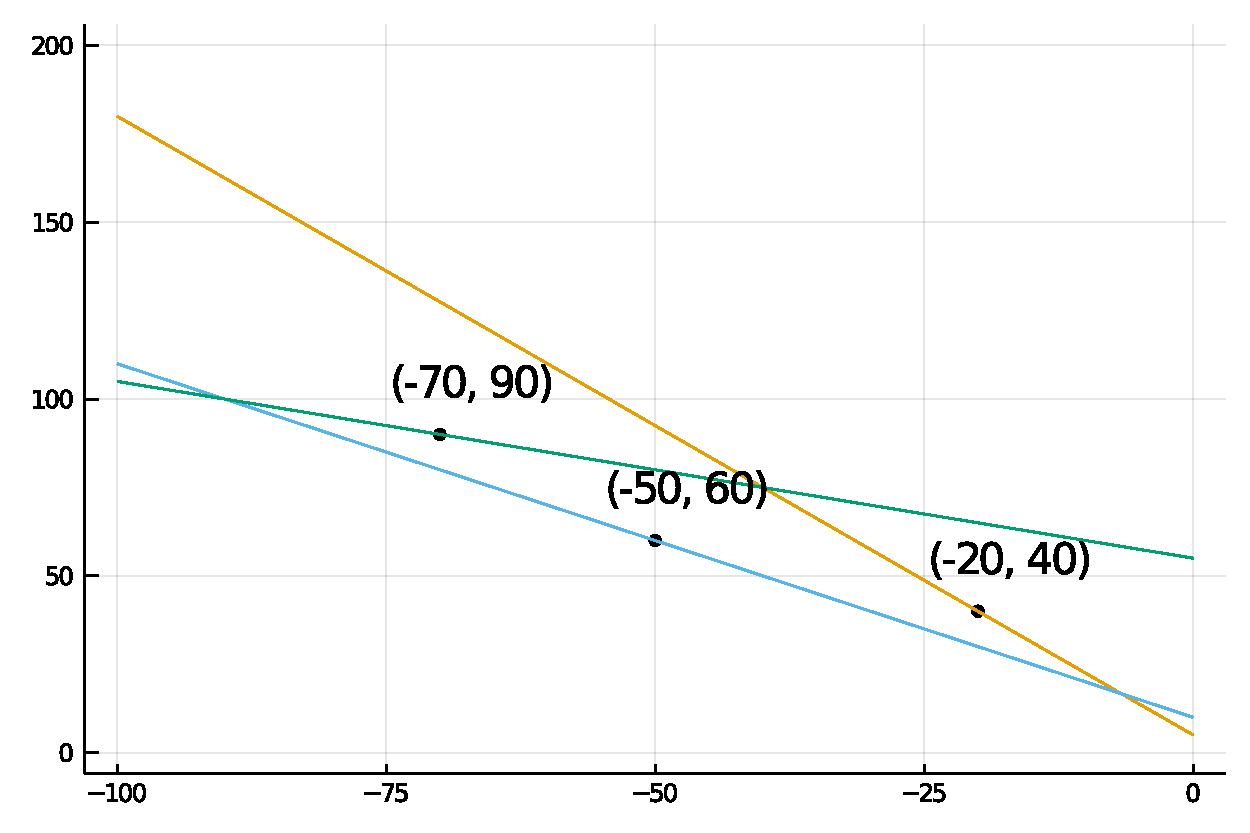
\includegraphics[width=0.97\textwidth]{Problem Set 1 Files/y_o_1.pdf}
    % \caption{Flower two.}
  \end{subfigure}
%   \caption{Punni no me quire nada bla bla }
\end{figure}



from the last graphic we can observe that the three observations are not consistent with a a  profit-maximizing firm; we observe that at price level $p=(5,5)$, the firm's choice is $y(p) = (-50,60)$ which gives a profit of $p\cdot y(p) = 50$ but

$$p\cdot (-20, 40) = p\cdot (-70, 90) = 100 > 50 $$

then, a profit-maximizing firm should have chosen any of those production plans instead of $y(p)$.

\textbf{Dataset 2}

We can draw the points $y(p)$ in the plane and the corresponding hyperplane for each price vector-production plan combination:

\begin{figure}[!htbp]
  \centering
  \begin{subfigure}{0.45\textwidth}
    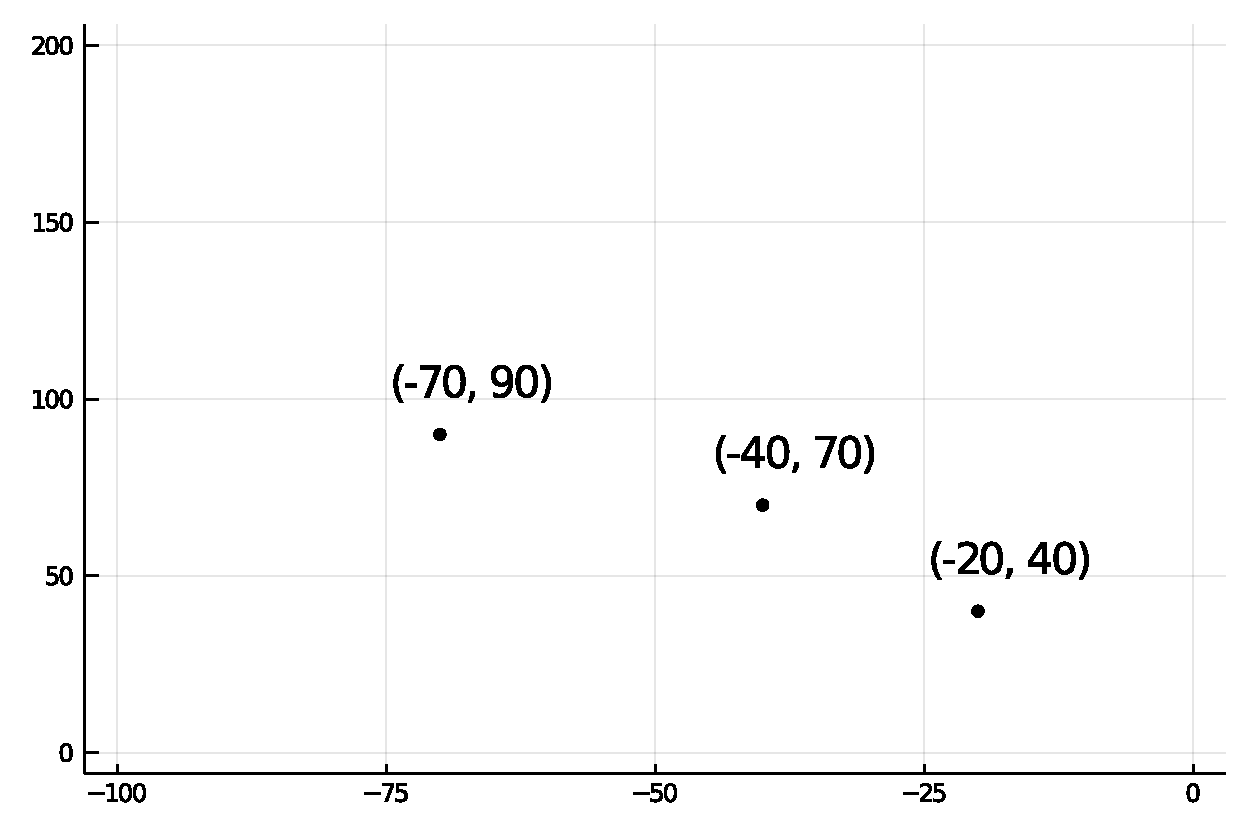
\includegraphics[width=0.97\textwidth]{Problem Set 1 Files/y_i_2.pdf}
    % \caption{Flower one.}
  \end{subfigure}
  \hfill
  \begin{subfigure}{0.45\textwidth}
    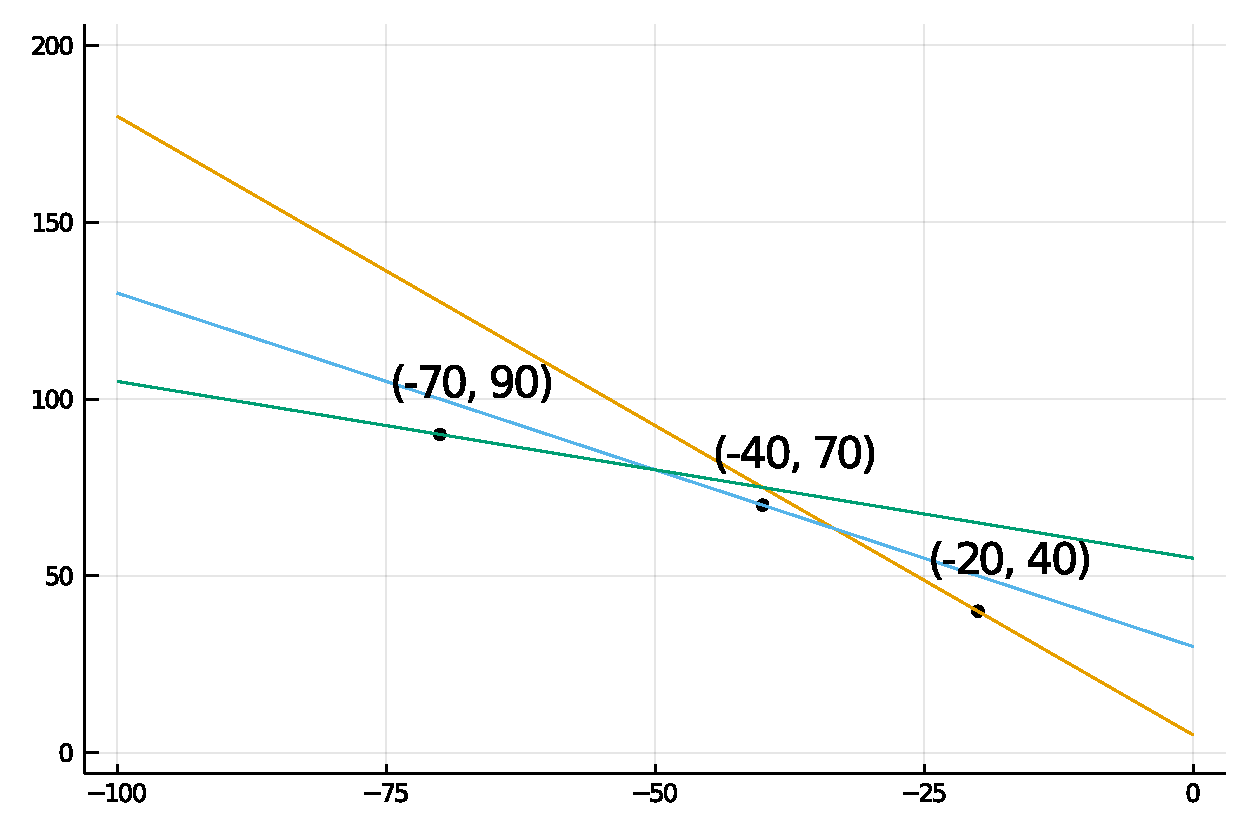
\includegraphics[width=0.97\textwidth]{Problem Set 1 Files/y_o_2.pdf}
    % \caption{Flower two.}
  \end{subfigure}
%   \caption{Punni me odia bla bla }
\end{figure}
the plot give us an indication that this set is rationalizable. For a formal proof consider the sets each the profits at each price vector-production plan combination:

$$(7,4) \cdot (-20,40)=20 \qquad
(5,5) \cdot (-40,70) = 100\qquad
(4,8) \cdot (-70,90) = 440$$

the Inner Bound:

$$Y^I = \{(-20,40), (-40,70), (-70,90) \}$$

and the Outer Bound:

$$Y^O = \{y\in\mathbb{R}^2 \settf y\cdot (7,4) \leq 20\} \cap \{y\in\mathbb{R}^2 \settf y\cdot (5,5) \leq 20\} \cap \{y\in\mathbb{R}^2 \settf y\cdot (4, 8) \leq 440\}$$

for each point in $Y^I$ we have:

$$(7,4) \cdot (-20,40)=20 \qquad  (7,4) \cdot (-40,70)=-70 \qquad (7,4) \cdot (-70,90)=-130$$
$$(5,5) \cdot (-20,40)=100 \qquad  (5,5) \cdot (-40,70)=150 \qquad (5,5) \cdot (-70,90)=100$$
$$(4,8) \cdot (-20,40)=240 \qquad  (4,8) \cdot (-40,70)=360 \qquad (4,8) \cdot (-70,90)=440

therefore $Y^I \subset Y^O$ thus proving that the observations are consistent with a profit-maximizing firm.

Now the sets the question ask for are the following:

\textbf{(a)} The the smallest production set that can rationalize the data is the Inner Bound $Y^I$, explicitly:

$$Y^I=\{(-20,40), (-40,70), (-70,90) \}$$

\textbf{(b)} The smallest convex production set with free disposal and the shutdown property that can rationalize the data.

First we need to include the production plan $(0,0)$. Since we are looking for a set with free disposal, we also need to consider the inner bound with free disposal (of our new set with $(0,0)$), this sett looks like this:
\begin{figure}[h]
    \centering
    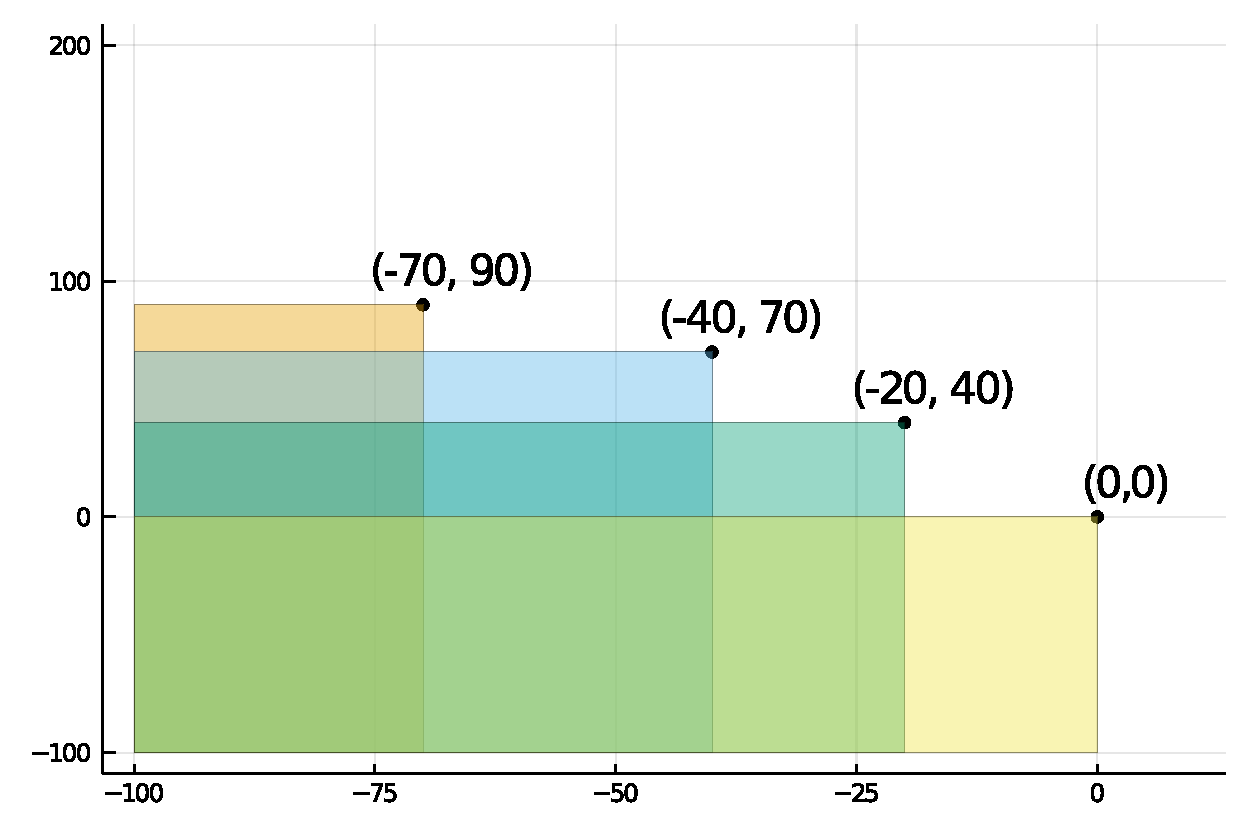
\includegraphics[scale=0.5]{Problem Set 1 Files/y_smallconvex_2.pdf}
    % \caption{Caption}
    \label{fig:my_label}
\end{figure}

We are looking for the smallest convex set (with free disposal), we need to add the least amount of points that make this set convex.

Consider the polygonal line that connects the corners in the previous set, if we add the missing triangles to the set we will get a convex production set with free disposal that looks like this:
\newpage
\begin{figure}[h]
    \centering
    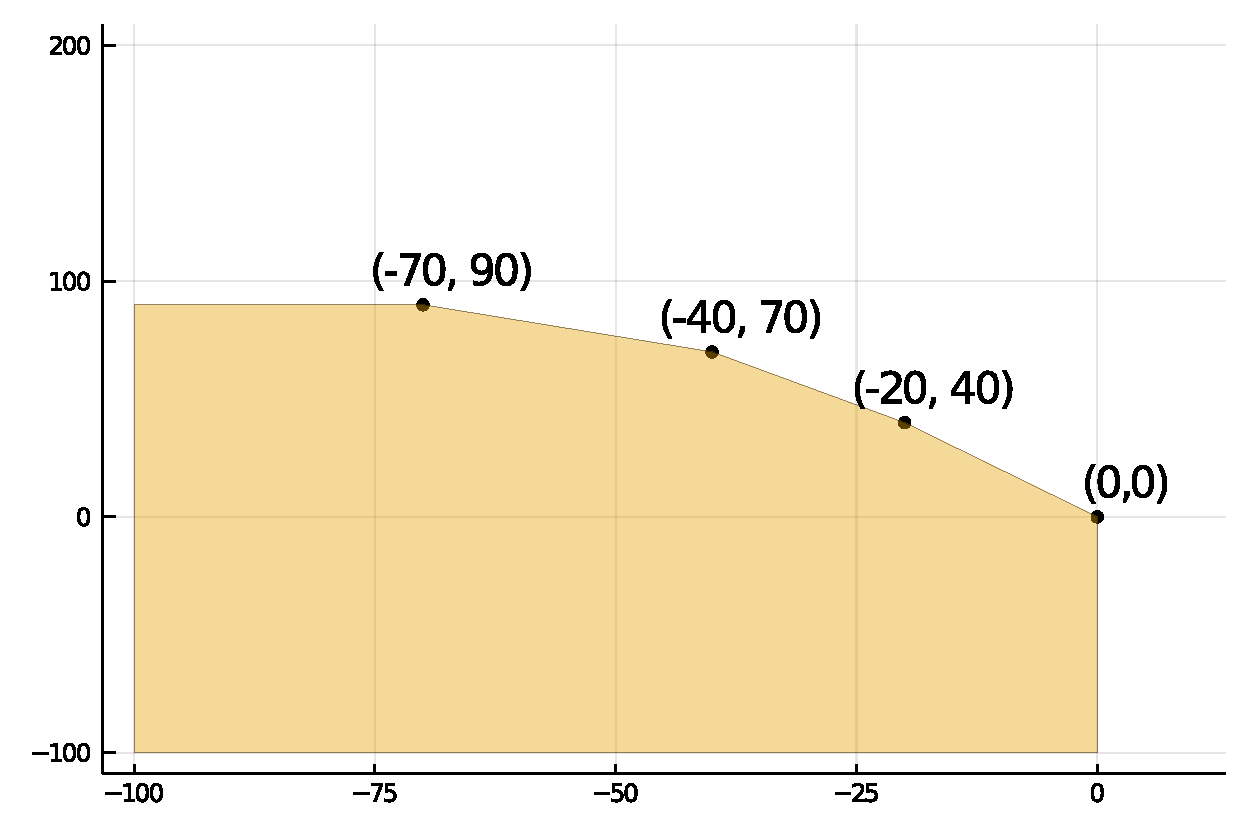
\includegraphics[scale=0.5]{Problem Set 1 Files/y_smallconvex_4.pdf}
    % \caption{Caption}
    \label{fig:my_label}
\end{figure}

by construction if we remove any point from this set it will cease to be convex, therefore this must be the set we are looking for.

\textbf{(c)} The largest production set that can rationalize the data is the Outer Bound $Y^O$, explicitly:

$$Y^O = \{y\in R^{2} \settf y\cdot (7,4) \leq 20\} \cap \{y\in R^{2} \settf y\cdot (5,5) \leq 150\} \cap \{y\in R^{2} \settf y\cdot (4,8) \leq 440\}$$

a graphic representation of this set is:
\begin{figure}[h]
    \centering
    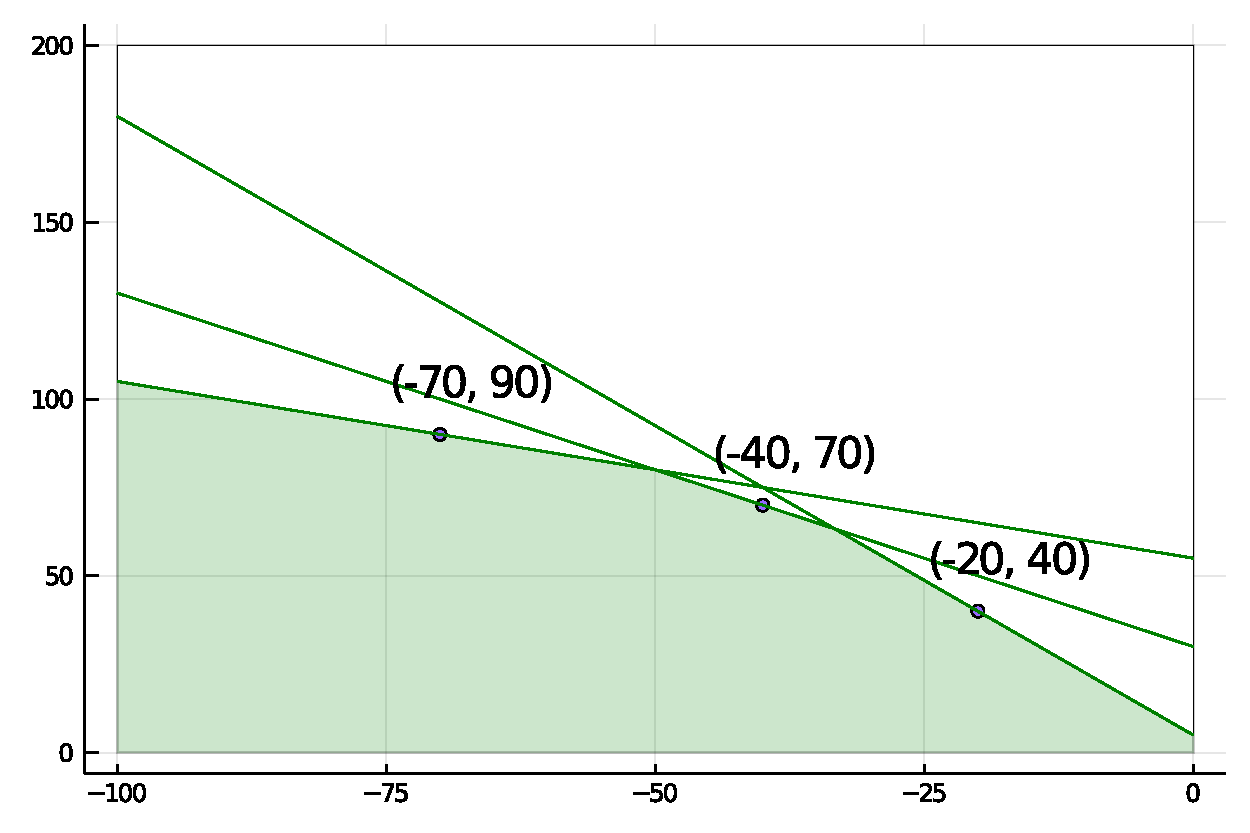
\includegraphics[scale=0.5]{Problem Set 1 Files/y_o_2_set.pdf}
    % \caption{Caption}
    \label{fig:my_label}
\end{figure}


\end{proof}

\begin{problem}[\textbf{Aggregate Production}]
Suppose an industry consists of $n$ profit-maximizing, price-taking firms, each with its own production set $Y_{1}, Y_{2}, \ldots, Y_{n}$. You observe industry-level data at several price vectors: instead of observing individual firm production $\left(y_{1}(p), y_{2}(p), \ldots, y_{n}(p)\right),$ you observe only the sum $y_{1}(p)+\ldots+y_{n}(p)$ Will this aggregate data satisfy the Weak Axiom? Can industry production be rationalized as if it were the choice of a single profit-maximizing firm? Explain. (You may find it helpful to use an example)
\end{problem}
\begin{proof}[Answer]

Let $y$ be an observation of the industry behavior when prices are $p$ and $y'$ when prices are $p'$ then we know that there are two sets:

$$\{y_i\}_{i=1}^n \qaq \{y_i\}_{i=1}^n$$

such that

$$y = \sum_{i=1}^n{y_i} \qquad y_i \in y_i(p)$$
$$y' = \sum_{i=1}^n{y'_i} \qquad y_i \in y_i(p')$$

Since every $Y_i$ is the production set of a profit-maximizing price taking firm, every data point from those sets must satisfy the Weak Axiom, then

\begin{align*}
    y\cdot p = \left(\sum_{i=1}^n{y_i}\right)p &= \sum_{i=1}^n{y_i}p
    \geq \sum_{i=1}^n{y'_i}p
    = \left(\sum_{i=1}^n{y'_i}\right)p = y'\cdot p 
\end{align*}

this means that

$$\boxed{\text{The aggregate data will satisfy the Weak Axiom. }}$$

To answer the question whether the Industry production data can be rationalized, consider first the Inner Bound of $Y$.Since every element of $Y$ must be the sum of elements of the $Y_i$ sets, we must have

$$Y^I \subseteq \sum_{i=1}^nY^I_i$$

Where the sum of sets is defined as the set that contains the sum of element of those sets

Now consider the outer bound of $Y$

$$Y^O = \bigcap_{p}\{y\in R^k\settf y\cdot p \leq y(p)\cdot p \} = \bigcap_{p}\{y\in R^k\settf y\cdot p \leq (y_i(p)+\ldots+y_n(p)) \cdot p \}$$

Fix any price $p$ and pick $y\in Y^I$,

\begin{align*}
    y\in Y^I &\qiq y =  \sum_{i=1}^n{y_i} \qaq y_i \in y_i(p)\\
    &\qiq y\cdott p =  \left(  \sum_{i=1}^n{y_i} \right)p =  \sum_{i=1}^n{y_i}p \leq \sum_{i=1}^n{y_i(p)p} = \left(\sum_{i=1}^n{y_i(p)}\right)p = y(p)p\\
\end{align*}

then

\begin{align*}
    y\in Y^I &\qiq y\in \bigcap_{p}\{y\in R^k\settf y\cdot p \leq y(p)\cdot p \} \quad \foorall\\
    &\qiq y \in Y^O\\
    &\qiq Y^I \subseteq Y^O
\end{align*}

then, by the result seen in class if the adding up condition is satisfied the data is rationalizable.

To see that the adding up condition is satisfied and complete the proof suppose that for the same price $p$ we observe two different values of industry production $y^1$ and $y^2$, with

$$ y^1\cdot p \neq y^2\cdot p$$

this is clearly impossible because this means that at least one firm is not maximizing profits which contradicts our assumptions.

\end{proof}

\end{document}
